\section{Prerequisitos}

\subsection{¿Qué es un contenedor?}

Un contenedor es una unidad estandarizada de software que empaqueta código y todas sus dependencias para que una aplicación se ejecute de forma rápida, confiable y consistente en diferentes entornos. Es una forma ligera, portátil y aislada de ejecutar procesos o aplicaciones.

\subsubsection{Componentes clave de un contenedor}
\begin{itemize}
    \item \textbf{Aplicación principal}: El binario o script que se quiere ejecutar.
    \item \textbf{Dependencias}: Librerías, módulos, herramientas del sistema necesarias.
    \item \textbf{Sistema de archivos aislado}: Un entorno controlado, consistente y separado del sistema operativo anfitrión.
    \item \textbf{Red y procesos aislados}: Gracias a tecnologías como \textit{cgroups} y \textit{namespaces} del kernel de Linux.
    \item \textbf{Capacidad de ser portado}: Se comporta igual en desarrollo, pruebas o producción.
\end{itemize}

\subsubsection{Creación y gestión de contenedores}
Para crear y gestionar contenedores, se utilizan herramientas como:

\paragraph{Docker:}
\begin{itemize}
    \item Permite construir imágenes (plantillas de contenedor) y lanzar contenedores a partir de ellas.
    \item Una \textit{imagen Docker} es como una instantánea de un sistema preconfigurado.
    \item Un \textit{contenedor Docker} es una instancia en ejecución de esa imagen.
\end{itemize}

\paragraph{Podman:}
\begin{itemize}
    \item Alternativa moderna a Docker, compatible con sus comandos, pero no necesita un \textit{daemon} (demonio) en segundo plano.
    \item Cada contenedor se ejecuta como un proceso del usuario, lo cual es más seguro en entornos multiusuario.
    \item Soporta \textit{rootless containers} (contenedores sin privilegios de administrador).
\end{itemize}

\subsubsection{¿Qué es Docker Compose?}
Docker Compose es una herramienta que permite definir y ejecutar múltiples contenedores Docker mediante un archivo YAML (\texttt{docker-compose.yml}). Es ideal para sistemas distribuidos o aplicaciones que requieren múltiples servicios, como una aplicación web con base de datos y servidor de caché.

\textbf{Ejemplo básico:}
\begin{lstlisting}[style=customstyle]
version: '3'
services:
  web:
    image: nginx
    ports:
      - "80:80"
  db:
    image: postgres
    environment:
      POSTGRES_PASSWORD: example
\end{lstlisting}

Este archivo lanza dos contenedores: uno con Nginx y otro con PostgreSQL, conectados en una red compartida automáticamente gestionada por Docker Compose.

\subsubsection{Diferencias entre Docker, Docker Compose y Podman}
\begin{table}[h!]
\centering
\begin{tabular}{|p{3cm}|p{3cm}|p{3cm}|p{3cm}|}
\hline
\textbf{Característica} & \textbf{Docker} & \textbf{Docker Compose} & \textbf{Podman} \\ \hline
Motor de contenedores & Sí & Usa Docker & Sí \\ \hline
Ejecuta múltiples contenedores & No directamente & Sí, orquestación básica & Sí, con \texttt{podman-compose} \\ \hline
Requiere daemon & Sí & Sí (usa Docker) & No \\ \hline
Rootless & Limitado & No & Sí, por diseño \\ \hline
Compatible con Dockerfiles & Sí & Sí & Sí \\ \hline
\end{tabular}
\end{table}

\subsubsection{Resumen conceptual}
Un contenedor no es una máquina virtual. No tiene su propio kernel ni simula hardware. Comparte el kernel del sistema anfitrión, lo que lo hace mucho más ligero y rápido, ideal para microservicios, DevOps y CI/CD.

Docker Compose y Podman son formas de gestionar contenedores: la primera, muy útil para múltiples servicios coordinados; la segunda, más flexible, más segura y sin necesidad de \textit{daemon}, orientada a usuarios avanzados y producción segura.

\subsection{Ejemplos}
\begin{itemize}
    \item Crear un contenedor con Docker: \texttt{docker run -d -p 80:80 nginx}
    \item Crear un contenedor con Podman: \texttt{podman run -d -p 80:80 nginx}
    \item Usar Docker Compose para lanzar múltiples servicios: \texttt{docker-compose up}
\end{itemize}

\subsubsection{Comparativa con una MV}

\subsubsection{Contenedor vs Máquina Virtual}

Tanto los contenedores como las máquinas virtuales aíslan aplicaciones del sistema anfitrión, pero lo hacen de formas muy diferentes.

\paragraph{Similitudes:}
Ambos permiten ejecutar aplicaciones en entornos separados, evitando que interfieran con el sistema principal.

\paragraph{Diferencias principales:}
\begin{table}[h!]
\centering
\begin{tabular}{|p{5cm}|p{5cm}|p{5cm}|}
\hline
\textbf{Característica}         & \textbf{Máquina Virtual}                     & \textbf{Contenedor}                     \\ \hline
Sistema Operativo               & Incluye su propio sistema operativo          & Comparte el kernel del anfitrión         \\ \hline
Peso                            & Pesado: varios GBs                           & Ligero: pocos MBs                        \\ \hline
Arranque                        & Lento (minutos)                              & Rápido (segundos o menos)                \\ \hline
Consumo de recursos             & Alto: CPU, RAM, disco                        & Bajo y eficiente                         \\ \hline
Virtualización                  & A nivel de hardware (hipervisor)             & A nivel de sistema operativo (namespaces) \\ \hline
Portabilidad                    & Limitada (por sistema operativo)             & Muy alta (misma imagen funciona en múltiples sistemas) \\ \hline
Ideal para                      & Emular sistemas completos, testing de OS     & Desarrollar y desplegar aplicaciones     \\ \hline
\end{tabular}
\end{table}

\paragraph{Analogía:}
Imagina un edificio:
\begin{itemize}
    \item Una máquina virtual es como un departamento completo: tiene su propio baño, cocina y sistema eléctrico. Es independiente, pero consume más recursos.
    \item Un contenedor es como una habitación en un mismo piso: tiene sus propios muebles y decoración (aplicación y dependencias), pero comparte el sistema de agua, luz y estructura (el kernel del sistema operativo).
\end{itemize}

\paragraph{Conclusión:}
Un contenedor es similar a una máquina virtual, pero más ligero y rápido porque no incluye un sistema operativo completo. Esto lo hace ideal para desarrollo, pruebas, despliegue continuo y microservicios.

\subsection{Instalación de Docker y Docker Compose}

A continuación, se presenta una guía detallada para instalar Docker y Docker Compose en Ubuntu 24.04, sin utilizar Docker Desktop, lo que resulta en una instalación más ligera y estable.

\subsubsection{1. Preparar el sistema}

Abra una terminal y actualice el sistema:

\begin{lstlisting}[style=customstyle]
sudo apt update && sudo apt upgrade -y
\end{lstlisting}

Instale las herramientas necesarias:

\begin{lstlisting}[style=customstyle]
sudo apt install ca-certificates curl gnupg lsb-release -y
\end{lstlisting}

\subsubsection{2. Agregar la clave GPG oficial de Docker}

Cree el directorio para almacenar la clave:

\begin{lstlisting}[style=customstyle]
sudo mkdir -p /etc/apt/keyrings
\end{lstlisting}

Descargue y almacene la clave GPG oficial de Docker:

\begin{lstlisting}[style=customstyle]
curl -fsSL https://download.docker.com/linux/ubuntu/gpg | sudo gpg --dearmor -o /etc/apt/keyrings/docker.gpg
\end{lstlisting}

\subsubsection{3. Agregar el repositorio oficial de Docker}

Agregue el repositorio de Docker a la lista de fuentes de APT:

\begin{lstlisting}[style=customstyle]
echo \
    "deb [arch=$(dpkg --print-architecture) signed-by=/etc/apt/keyrings/docker.gpg] \

    https://download.docker.com/linux/ubuntu \
    $(lsb_release -cs) stable" | \
    sudo tee /etc/apt/sources.list.d/docker.list > /dev/null
\end{lstlisting}

\subsubsection{4. Instalar Docker Engine y Docker Compose}

\textbf{Nota: Es para nuestra máquina (ubuntu).}

Actualice los paquetes e instale Docker y Docker Compose:

\begin{lstlisting}[style=customstyle]
sudo apt update
sudo apt install docker-ce docker-ce-cli containerd.io docker-buildx-plugin docker-compose-plugin -y
\end{lstlisting}

\subsubsection{5. Verificar que Docker está funcionando}

Ejecute los siguientes comandos para verificar la instalación:

\begin{lstlisting}[style=customstyle]
sudo docker version
sudo docker info
\end{lstlisting}

Si se muestra información sobre Docker, la instalación fue exitosa.

\subsubsection{6. (Opcional) Ejecutar Docker sin \texttt{sudo}}

Para permitir que Docker se ejecute sin necesidad de usar \texttt{sudo}, ejecute:

\begin{lstlisting}[style=customstyle]
sudo usermod -aG docker $USER
\end{lstlisting}


Acto seguido, cierre la sesión y vuelva a iniciarla para que los cambios surtan efecto.
\begin{lstlisting}[style=customstyle]
sudo systemctl restart docker
\end{lstlisting}

\textbf{Nota:} Cierre la sesión y vuelva a iniciarla (o reinicie el sistema) para que los cambios surtan efecto.

\subsection{Guía rápida de prueba}

\subsubsection{1. Probar Docker}

Ejecute el siguiente comando para probar Docker:

\begin{lstlisting}[style=customstyle]
docker run hello-world
\end{lstlisting}

Debería aparecer un mensaje indicando que Docker está instalado correctamente.

\subsubsection{2. Probar Docker Compose}

Cree una carpeta de prueba y acceda a ella:

\begin{lstlisting}[style=customstyle]
mkdir docker-prueba && cd docker-prueba
\end{lstlisting}

Cree un archivo \texttt{docker-compose.yml}:

\begin{lstlisting}[style=customstyle]
nano docker-compose.yml
\end{lstlisting}

Pegue el siguiente contenido en el archivo:

\begin{lstlisting}[style=customstyle]
version: "3.8"
services:
    web:
        image: nginx
        ports:
            - "8080:80"
\end{lstlisting}

Guarde y cierre el archivo. Luego, ejecute el servicio:

\begin{lstlisting}[style=customstyle]
docker compose up -d
\end{lstlisting}

Abra un navegador y acceda a \texttt{http://localhost:8080}. Debería visualizar la página de bienvenida de NGINX.

Para detener el servicio, ejecute:

\begin{lstlisting}[style=customstyle]
docker compose down
\end{lstlisting}

Con estos pasos, Docker y Docker Compose estarán instalados y funcionando correctamente.

\subsection{Instalación de Docker Engine en Rocky Linux 9 (o CentOS Stream 9)}

Esta guía es ideal para máquinas virtuales (MV) sin entorno gráfico.

\subsubsection{Paso 1: Preparar el sistema}

Actualice el sistema con los siguientes comandos:

\begin{lstlisting}[style=customstyle]
sudo dnf update -y
sudo dnf upgrade -y
\end{lstlisting}

Instale los paquetes necesarios:

\begin{lstlisting}[style=customstyle]
sudo dnf install -y dnf-utils device-mapper-persistent-data lvm2
\end{lstlisting}

\subsubsection{Paso 2: Agregar el repositorio oficial de Docker}

Agregue el repositorio oficial de Docker con el siguiente comando:

\begin{lstlisting}[style=customstyle]
sudo dnf config-manager --add-repo https://download.docker.com/linux/centos/docker-ce.repo
\end{lstlisting}

\textbf{Nota:} Docker no ofrece repositorios específicos para Rocky Linux, pero el de CentOS funciona perfectamente.

\subsubsection{Paso 3: Instalar Docker Engine}

Instale Docker Engine y sus componentes:

\begin{lstlisting}[style=customstyle]
sudo dnf install -y docker-ce docker-ce-cli containerd.io docker-buildx-plugin docker-compose-plugin
\end{lstlisting}

\subsubsection{Paso 4: Habilitar y arrancar el servicio Docker}

Habilite y arranque el servicio Docker con los siguientes comandos:

\begin{lstlisting}[style=customstyle]
sudo systemctl enable docker
sudo systemctl start docker
\end{lstlisting}

\subsubsection{Paso 5: Verificar la instalación}

Verifique que Docker se instaló correctamente ejecutando:

\begin{lstlisting}[style=customstyle]
docker --version
\end{lstlisting}

Debería mostrar una salida similar a:

\texttt{Docker version 24.x.x, build xxxxxxx}

\subsubsection{Paso 6: Permitir el uso de Docker a usuarios no root}

Para permitir que Docker se ejecute sin necesidad de usar \texttt{sudo}, siga estos pasos:

\begin{enumerate}
    \item Cree el grupo \texttt{docker} (si no existe):
    \begin{lstlisting}[style=customstyle]
sudo groupadd docker
    \end{lstlisting}
    \item Añada su usuario al grupo:
    \begin{lstlisting}[style=customstyle]
sudo usermod -aG docker $USER
    \end{lstlisting}
    \item Cierre la sesión y vuelva a iniciarla para aplicar los cambios.
\end{enumerate}

Pruebe que Docker se ejecuta sin \texttt{sudo} ejecutando:

\begin{lstlisting}[style=customstyle]
docker run hello-world
\end{lstlisting}


\section{Microservicios}

La arquitectura de microservicios es un enfoque de desarrollo de software en el que una aplicación se descompone en un conjunto de pequeños servicios independientes que se comunican entre sí mediante APIs o sistemas de mensajería como RabbitMQ, Kafka o Qpid. Cada microservicio está diseñado para encargarse de una funcionalidad específica del sistema y puede desarrollarse, desplegarse y escalarse de manera autónoma.

Este modelo ha ganado popularidad con el auge de los contenedores, ya que facilita el despliegue y la gestión de estos servicios de forma independiente. Entre sus principales ventajas destacan:

\begin{itemize}
    \item \textbf{Flexibilidad:} Cada servicio puede utilizar su propio stack tecnológico, adaptándose mejor a sus necesidades específicas.
    \item \textbf{Escalabilidad:} Permite escalar verticalmente (mejorando los recursos de un servicio) u horizontalmente (añadiendo instancias del servicio según la demanda).
\end{itemize}

Para más información sobre esta arquitectura, se recomienda consultar el artículo de Martin Fowler: \href{https://martinfowler.com/articles/microservices.html}{Microservices}.

\section{Ejercicio Evaluable. Ejecutar “Hello World”}

Instale Docker en su ordenador anfitrión o en una MV y ejecute el contenedor
``Hello World'' disponible en: \href{https://hub.docker.com/_/hello-world}.

Para ello debemos de ejecutar los siguientes comandos:

\begin{enumerate}[label=\textbf{\arabic*:}]
    \item \micode{sudo docker version}: para ver si docker está instalado correctamente.
    \item \micode{sudo docker run hello-world}: para ejecutar el contenedor. (Ver figura \ref{fig:hello-world})
\end{enumerate}

\begin{figure}[H]
    \centering
    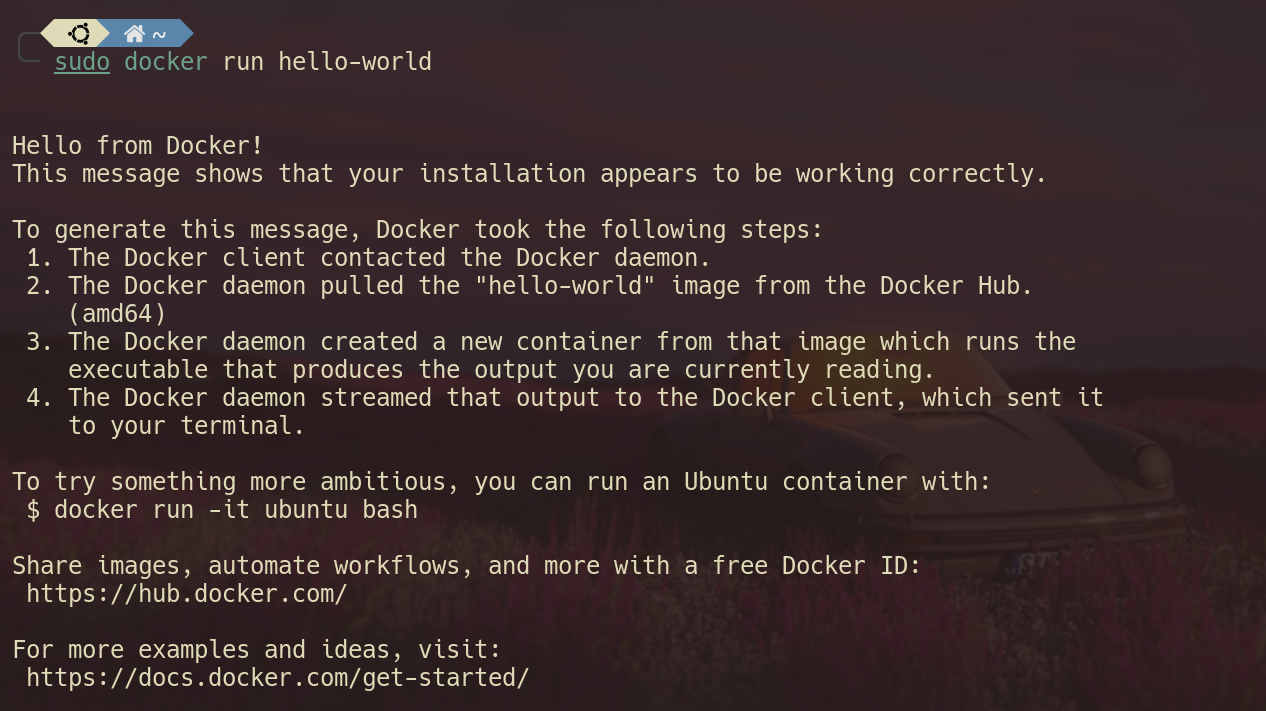
\includegraphics[width=0.8\textwidth]{images/Bloque2/hello-world.png}
    \caption{Contenedor Hello World}
    \label{fig:hello-world}
\end{figure}

\section{BenchMarks}

\subsection{¿Qué es un Benchmark?}

Un \textit{benchmark} es una prueba diseñada para medir el rendimiento de un sistema, componente o servicio informático. Estas pruebas pueden evaluar diversos aspectos, como velocidad, eficiencia, capacidad de respuesta o consumo de recursos. Existen múltiples tipos de \textit{benchmarks}, cada uno enfocado en un área específica del sistema.

Por ejemplo, para evaluar el rendimiento de un servidor DNS (que traduce nombres de dominio a direcciones IP), se pueden utilizar herramientas como \texttt{NameBench} o \texttt{GRC’s DNS Benchmark}, las cuales están diseñadas con pruebas estándar para este tipo de servicio.

\subsection{¿Por qué crear un Benchmark propio?}

Aunque existen herramientas predefinidas para realizar \textit{benchmarks}, en ocasiones es necesario programar uno propio para analizar parámetros específicos que no estén cubiertos por las herramientas existentes. Para ello, es importante considerar los siguientes elementos:

\begin{itemize}
    \item \textbf{Objetivo del Benchmark:} Definir claramente qué se desea medir, como latencia, \textit{throughput}, uso de CPU, etc.
    \item \textbf{Métricas:} Establecer las medidas que se utilizarán para evaluar el rendimiento. Esto incluye:
    \begin{itemize}
        \item Las unidades de medida (por ejemplo, milisegundos, MB/s).
        \item Las variables a observar (por ejemplo, tiempo de respuesta, carga del sistema).
        \item El método para calcular los resultados finales.
    \end{itemize}
    \item \textbf{Instrucciones de uso:} Especificar cómo ejecutar el \textit{benchmark}, el entorno requerido y los parámetros necesarios.
    \item \textbf{Ejemplo de uso y análisis de resultados:} Incluir una prueba real, interpretar los datos obtenidos y extraer conclusiones relevantes.
\end{itemize}

\subsection{OpenBenchmarking y Phoronix Test Suite (PTS)}

\subsubsection{OpenBenchmarking}

\textit{OpenBenchmarking} es un repositorio de \textit{benchmarks} de código abierto que permite a los usuarios utilizar, modificar o crear nuevas pruebas basadas en las existentes. Es una excelente fuente de inspiración para desarrollar \textit{benchmarks} personalizados.

\subsubsection{Phoronix Test Suite (PTS)}

\textit{Phoronix Test Suite (PTS)} es una plataforma asociada a \textit{OpenBenchmarking} que facilita la ejecución de \textit{benchmarks}. Es una herramienta versátil y popular para realizar pruebas de rendimiento en sistemas Linux, Windows o incluso en máquinas virtuales (MVs). Entre sus características destacan:

\begin{itemize}
    \item Amplia variedad de pruebas disponibles que se pueden ejecutar directamente desde su entorno.
    \item Integración con \textit{OpenBenchmarking}, lo que permite comparar resultados con otras máquinas.
    \item Compatibilidad con múltiples entornos, incluyendo contenedores Docker.
\end{itemize}

\subsubsection{Instalación de Phoronix Test Suite (PTS)}

La instalación de \textit{PTS} varía según el entorno utilizado:

\begin{itemize}
    \item En sistemas Debian/Ubuntu, se pueden usar paquetes precompilados.
    \item En máquinas virtuales con Rocky Linux, se recomienda el instalador universal para Linux.
    \item En Windows, también se ofrece soporte de instalación.
    \item Para las prácticas, la opción más recomendada es utilizar contenedores Docker.
\end{itemize}

\subsubsection{Enlaces útiles}

A continuación, se presentan enlaces relevantes para explorar más sobre \textit{benchmarks} y herramientas asociadas:

\begin{itemize}
    \item Software relacionado con \textit{benchmarks} en Linux: \\
    \href{https://sourceforge.net/directory/linux/?q=benchmark}{sourceforge.net/directory/linux/?q=benchmark}
    \item Repositorio de OpenBenchmarking: \href{https://openbenchmarking.org/}{openbenchmarking.org}
    \item Sitio web de Phoronix Test Suite: \href{https://www.phoronix-test-suite.com/}{phoronix-test-suite.com}
    \item Página de descargas de PTS: \href{https://www.phoronix-test-suite.com/?k=downloads}{phoronix-test-suite.com/?k=downloads}
    \item Imagen Docker recomendada para las prácticas: \href{https://hub.docker.com/r/phoronix/pts/}{hub.docker.com/r/phoronix/pts/}
\end{itemize}

\subsection{Ejercicio Opcional. Ejecutar un Benchmark}

El alumno/a debe ser capaz de utilizar \textit{Phoronix Test Suite} para:

\begin{itemize}
    \item Descargar, instalar y ejecutar un \textit{benchmark} de su elección.
    \item Almacenar y recuperar los resultados de múltiples ejecuciones del \textit{benchmark}.
    \item Explicar el objetivo del \textit{benchmark} y de los resultados obtenidos.
\end{itemize}

\subsubsection*{Solución con un benchmark distinto}

En mi caso en el propio enlace que nos ofrece la guía\footnote{\url{https://sourceforge.net/directory/linux/?q=benchmark}} he optado por instalar el que benchmarck que tiene como nombre benchmark\footnote{\url{https://sourceforge.net/projects/benchmark.mirror/}} y estoy siguiendo los pasos que aparecen en el fichero \textit{Readme.md}\footnote{Lo estoy instalando en mi máquina anfitrión.}.

Los pasos que he seguido se puede ver en la figura \ref{fig:benchmark}.

\begin{figure}[H]
    \centering
    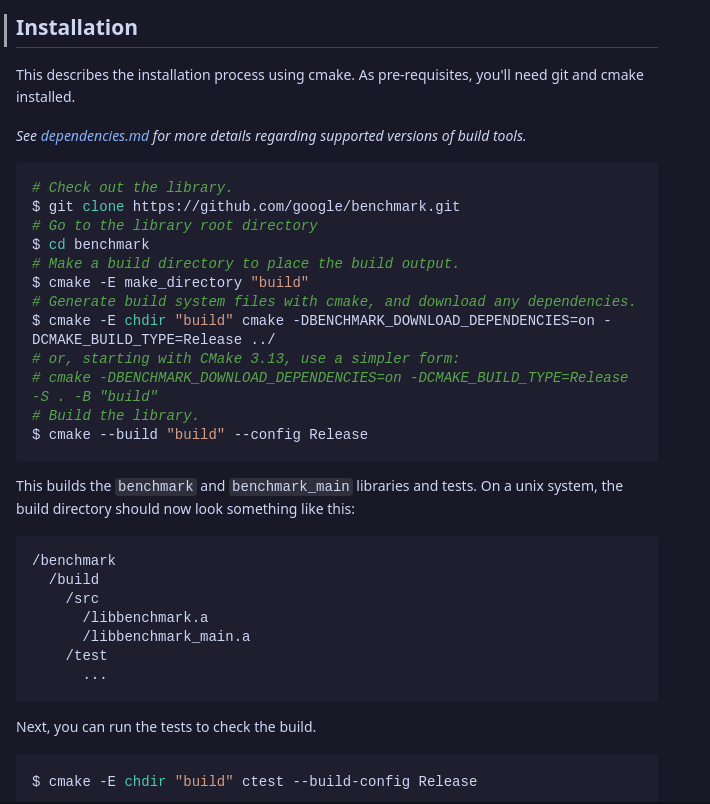
\includegraphics[width=0.8\textwidth]{images/Bloque2/installationBench.png}
    \caption{Instalación de benchmark}
    \label{fig:benchmark}
\end{figure}

Y el resultado del comando de ejecución de los tests lo puede ver en la figura \ref{fig:benchmarkResult}.

\begin{figure}[H]
    \centering
    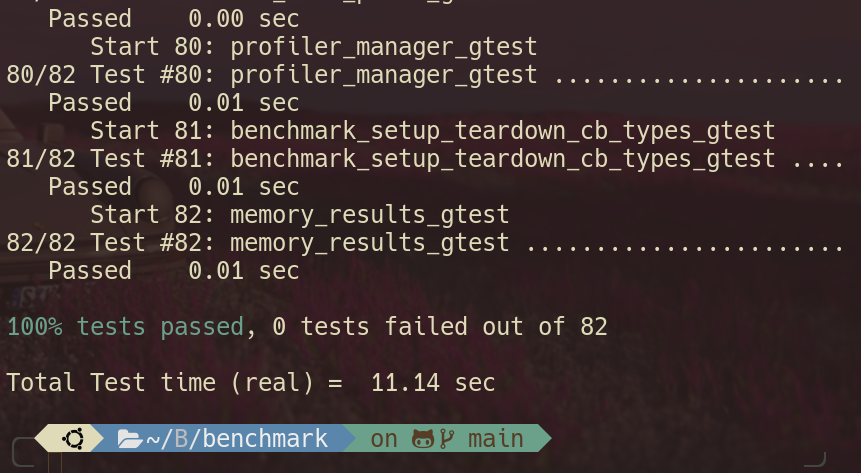
\includegraphics[width=0.8\textwidth]{images/Bloque2/resultsBench.png}
    \caption{Resultado de la ejecución del benchmark}
    \label{fig:benchmarkResult}
\end{figure}

A continuación, instalamos las librerias globales y probamos con el fichero básico que nos proporcioan, compilando y demás, nos da la salida que podemos ver en la figura \ref{fig:benchmarkResult2}.

\begin{figure}[H]
    \centering
    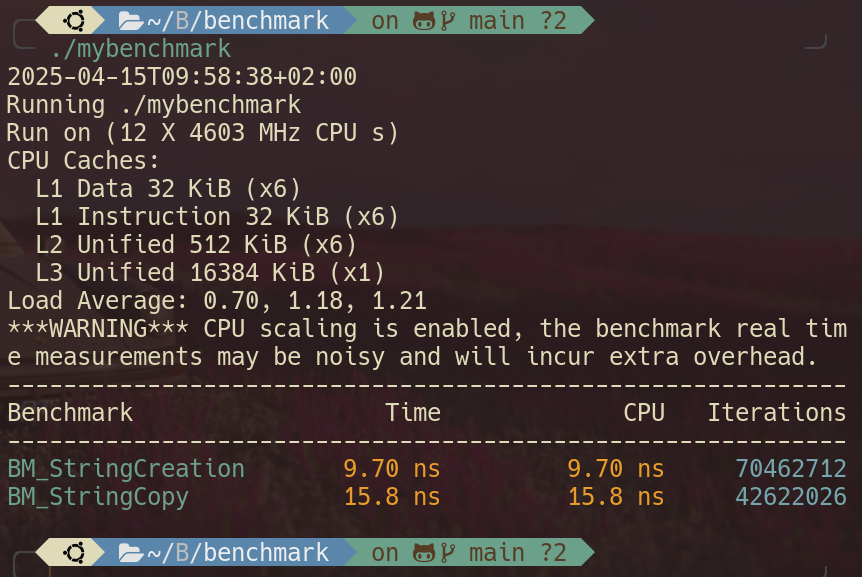
\includegraphics[width=0.8\textwidth]{images/Bloque2/resultsMYBENCHMARK.png}
    \caption{Resultado de la ejecución del benchmark}
    \label{fig:benchmarkResult2}
\end{figure}

\subsection*{Solución usando el benchmark que se especifica}

Para ello me he descargado el zip de la web y como estoy en Linux he ejecutado el comando \micode{sudo ./install.sh} y me ha instalado el programa en la ruta \micode{/usr/bin/phoronix-test-suite}.
\begin{figure}[H]
    \centering
    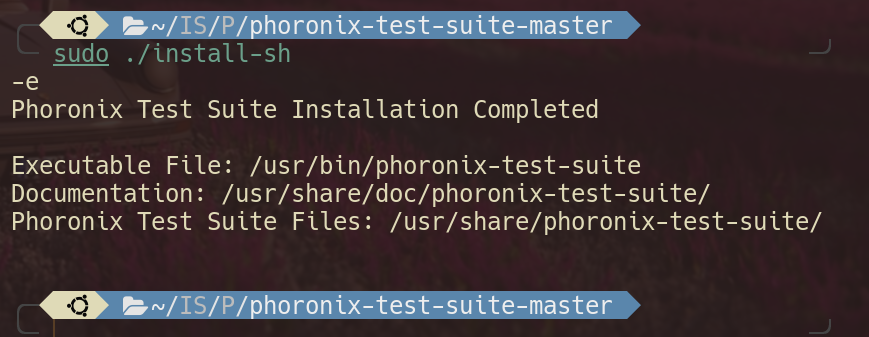
\includegraphics[width=0.8\textwidth]{images/Bloque2/installPhoro.png}
    \caption{Instalación de Phoronix Test Suite}
    \label{fig:PTS}
\end{figure}

Debemos de leer el Readme para una prueba.

En base a \textit{``phoronix-test-suite benchmark smallpt to run a simple CPU test
profile''} introducimos el comando para un primer testeo. 

% \includepdf[nup=2x2, pages=1-3, frame=true]{"../../Ficheros_Ejercicios/Ejercicios_Bloque2/resultsfirststatement.pdf"}

Donde el resultado que nos da:

\begin{lstlisting}[style=customstyle]
    resultsFirstAttempt
results


results: 

	Processor: AMD Ryzen 5 7535HS @ 4.60GHz (6 Cores / 12 Threads), Motherboard: ASUS TUF Gaming A15 FA506NC_FA506NC FA506NC v1.0 (FA506NC.308 BIOS), Chipset: AMD 17h-19h PCIe Root Complex, Memory: 2 x 8GB DDR5-4800MT/s Samsung M425R1GB4PB0-CWMOL, Disk: 512GB SAMSUNG MZVL8512HELU-00BTW + 1000GB KINGSTON SNV3S1000G, Graphics: ASUS NVIDIA GeForce RTX 3050 Mobile, Audio: NVIDIA Device 2291, Network: Realtek RTL8111/8168/8211/8411 + Realtek RTL8852BE PCIe 802.11ax

	OS: Ubuntu 24.04, Kernel: 6.11.0-21-generic (x86_64), Display Server: X Server, Compiler: GCC 13.3.0, File-System: ext4, Screen Resolution: 1920x1080


Smallpt 1.0
Global Illumination Renderer; 128 Samples
Seconds < Lower Is Better
results . 15.48 |==============================================================

\end{lstlisting}

% Otro de los benchmarks que podemos ejecutar es ``unigine-heaven''. Para ello debemos de ejecutar los comandos \micode{./phoronix-test-suite install unigine-heaven; ./phoronix-test-suite run unigine-heaven}


\subsection{Resumen: Phoronix Test Suite en Máquina Local vs Docker}

El \textit{Phoronix Test Suite} puede presentar problemas de rendimiento o fallos en una máquina local debido a dependencias faltantes, configuraciones incorrectas o conflictos en el entorno del sistema operativo. En contraste, al ejecutarlo en un contenedor Docker, se utiliza un entorno limpio y preconfigurado, optimizado por los desarrolladores para funcionar de manera eficiente.

\subsubsection{Comparativa entre Máquina Local y Docker}

\begin{table}[h!]
\centering
\begin{tabular}{|p{4cm}|p{5cm}|p{5cm}|}
\hline
\textbf{Aspecto} & \textbf{Máquina Local} & \textbf{Contenedor Docker} \\ \hline
PHP y extensiones & Puede faltar GD, bzip2, sqlite3, etc. & Todo preinstalado y configurado \\ \hline
Permisos y acceso a GPU & Problemas con \texttt{/dev/dri} u otros permisos & Aislado, puede no usar GPU directamente \\ \hline
Entorno gráfico & Falta de X11 puede romper tests gráficos & Usa \textit{fallback} o modo \textit{headless} \\ \hline
Dependencias del sistema & Conflictos o paquetes rotos & Imagen oficial limpia y probada \\ \hline
Compatibilidad de librerías & Incompatibilidades posibles & Versiones probadas y compatibles \\ \hline
\end{tabular}
\caption{Comparativa entre ejecución local y en Docker}
\end{table}

\subsubsection{Caso Específico: Benchmark \texttt{smallpt}}

El \texttt{smallpt} es un \textit{benchmark} dependiente de la CPU. Problemas como \textit{throttling}, gestión térmica deficiente o extensiones PHP faltantes pueden ralentizar su ejecución en una máquina local. En Docker, estos problemas se mitigan gracias al entorno controlado.

\subsubsection{Ventajas de Docker}

\begin{itemize}
    \item Entorno aislado y preconfigurado.
    \item Independencia de configuraciones locales.
    \item Fácil reinicio y limpieza del entorno.
    \item Uso de versiones probadas por los desarrolladores.
\end{itemize}

En resumen, ejecutar \textit{Phoronix Test Suite} en Docker garantiza mayor estabilidad y rendimiento, eliminando problemas derivados del entorno local.



Realizando diversas pruevas vemos que el comando tarda demasiado y con htop vemos que no se queda colgado pero tarda demasiado tiempo, por ende, he decidido ejecutarlo en contenedores que es como se recomienda en prácticas. 


Para ello ejecutamos los siguientes comandos:

\begin{enumerate}
    \item \micode{docker pull phoronix/pts}: para descargar la imagen de Phoronix Test Suite\footnote{El comando es de la \url{https://www.phoronix-test-suite.com/?k=downloads}.}.
    \item \micode{docker run -it --rm phoronix/pts}: para ejecutar el contenedor interactivo.
    \item \micode{phoronix-test-suite benchmark smallpt}: para ejecutar el benchmark.
\end{enumerate}

De manera que una vez que estamos dentro de la shell interactiva del docker podemos ejecutar los comandos del docker.

Los pasos a seguir para los tests son (dentro del docker de phoronix con la shell interactiva):
\begin{enumerate}
    \item Listamos los disponibles usando el comando \micode{list-avilable-test}
    \item install <test>
    \item run <test>
\end{enumerate}

En mi caso con he instalado el test \micode{php}. El resultado podemos verlo en la terminal (Ver figura \ref{fig:dockerPhoronix}). Además tenemos la opción de subirlo y poder consultarlo de manera online, en mi caso es \url{https://openbenchmarking.org/result/2504152-NE-RESULTSPH66}.

\begin{figure}[H]
    \centering
    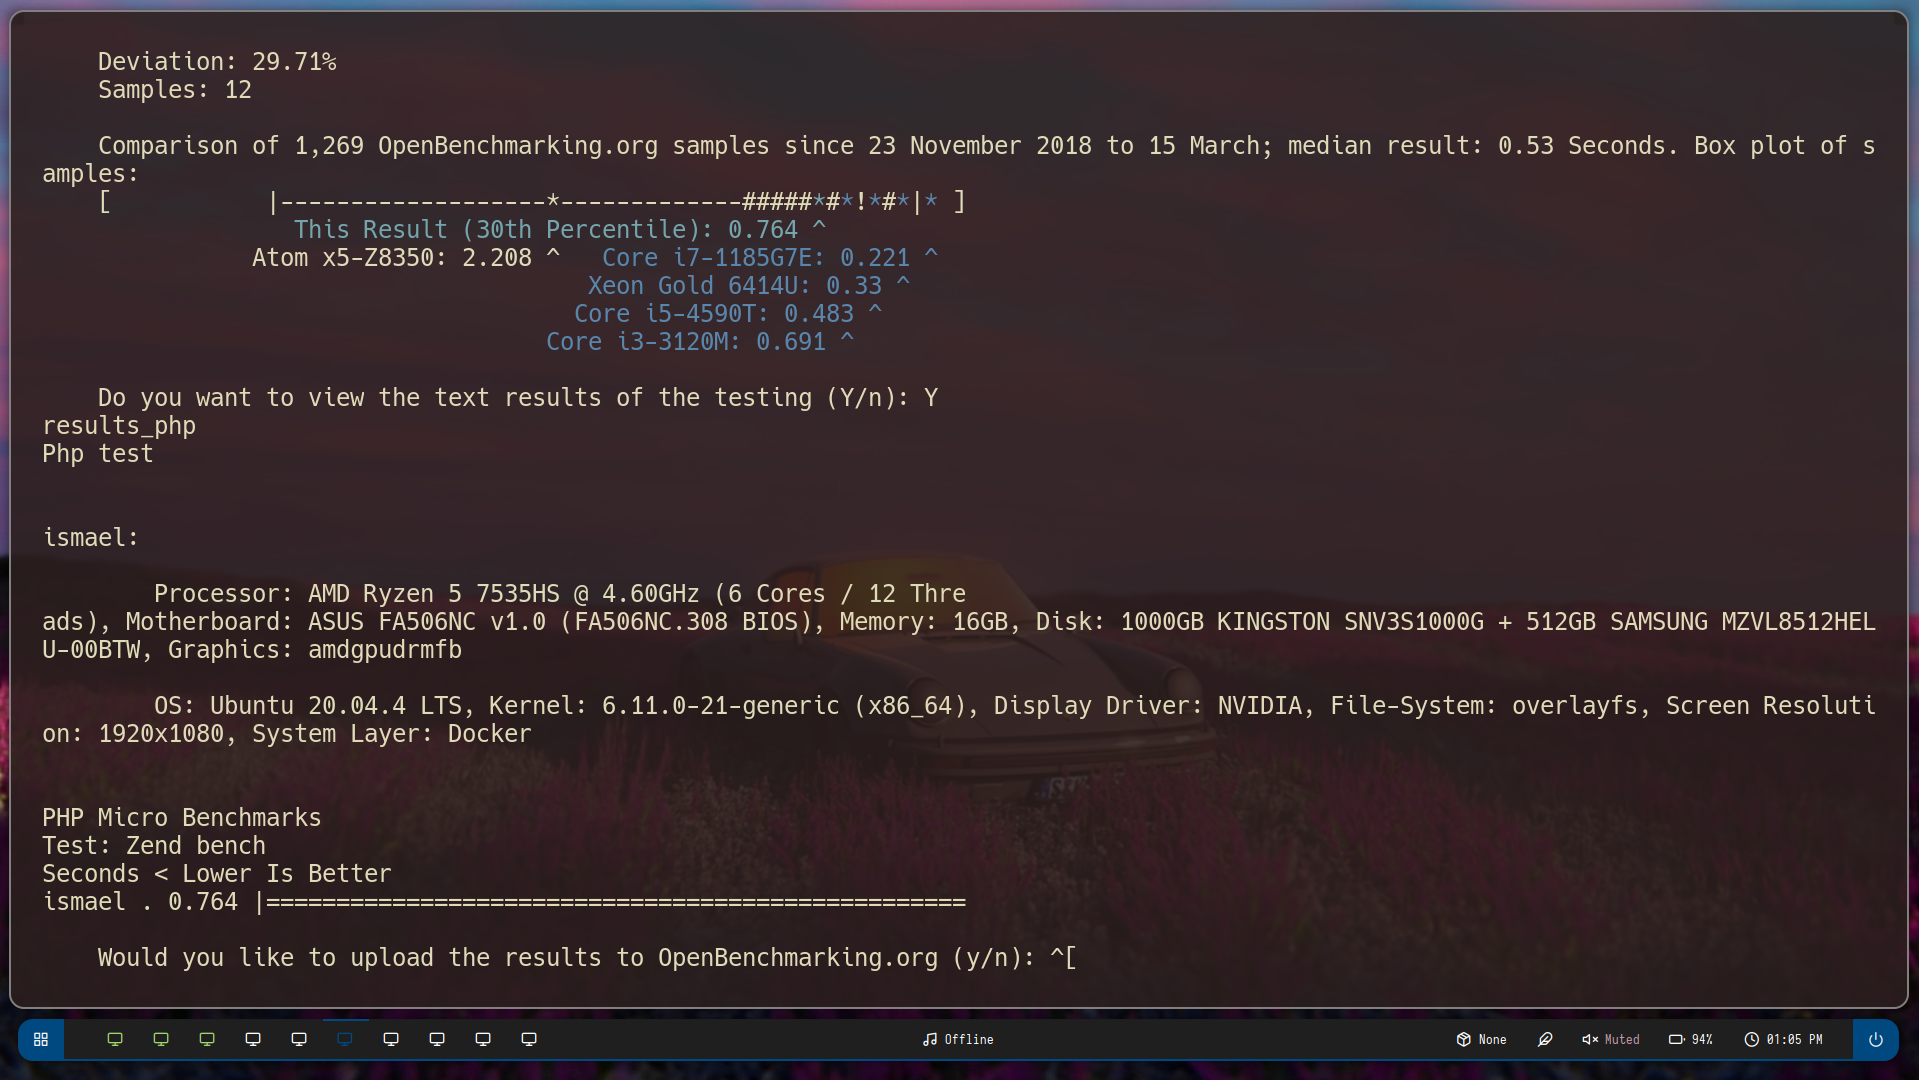
\includegraphics[width=1\textwidth]{images/Bloque2/dockerPhoronix.png}
    \caption{Resultado de la ejecución del benchmark en Docker}
    \label{fig:dockerPhoronix}
\end{figure}

\subsection*{Objetivo del Benchmark y Resultados Obtenidos}

El objetivo del benchmark realizado con \textbf{Phoronix Test Suite} fue evaluar el rendimiento del sistema, específicamente en la ejecución de pruebas micro de \textbf{PHP Zend}, bajo condiciones estándar. Este tipo de pruebas mide la eficiencia y tiempos de ejecución de componentes clave, como el procesador y la memoria, proporcionando una comparación con otros sistemas.

\subsubsection{Resultados Obtenidos}

\begin{itemize}
    \item \textbf{Tiempo promedio de ejecución}: 0.764 segundos.
    \item \textbf{Desviación estándar}: SE +/- 0.066, lo que indica una alta consistencia en los resultados.
    \item \textbf{Percentil alcanzado}: No especificado, pero los resultados muestran un rendimiento competitivo en comparación con sistemas similares.
\end{itemize}

\subsubsection{Interpretación de los Resultados}

El sistema probado, con un procesador AMD Ryzen 5 7535HS, mostró un rendimiento destacado en las pruebas de PHP Zend, con tiempos de ejecución significativamente bajos. Esto lo posiciona como una opción eficiente para entornos que requieren alta velocidad y confiabilidad en la ejecución de aplicaciones web o API basadas en PHP.

\subsubsection{Conclusión}

El benchmark confirma que el sistema es altamente eficiente en tareas relacionadas con PHP, siendo una opción ideal para desarrolladores y administradores de sistemas que buscan optimizar el rendimiento de sus servidores o aplicaciones en entornos de producción.







